\chapter{2012年新课标卷（文）}

\section{单选题}

\begin{problem}
已知集合 \(A = \{x \mid x^2 - x - 2 < 0\}\)，\(B = \{x \mid -1 < x < 1\}\)，则（\quad）

\choices
    {\(A \subsetneq B\)}
    {\(B \subsetneq A\)}
    {\(A = B\)}
    {\(A \cap B = \varnothing\)}
\end{problem}

\begin{problem}
复数 \(z = \frac{-3 + \i}{2 + \i}\) 的共轭复数是（\quad）

\choices
    {\(2 + \i\)}
    {\(2 - \i\)}
    {\(-1 + \i\)}
    {\(-1 - \i\)}
\end{problem}

\begin{problem}
在一组样本数据 \((x_{1}, y_{1})\)，\((x_{2}, y_{2})\)，\(\cdots\)，\((x_{n}, y_{n})\) （\(n \geqslant 2\)，\(x_{1}\)，\(x_{2}\)，\(\cdots\)，\(x_{n}\) 不全相等） 的散点图中，若所有样本点 \((x_{i}, y_{i}) (i = 1, 2, \cdots, n)\) 都在直线 \(y = \frac{1}{2} x + 1\) 上，则这组样本数据的样本相关系数为（\quad）

\choices
    {\(-1\)}
    {0}
    {\( \frac{1}{2} \)}
    {1}
\end{problem}

\begin{problem}
设 \(F_{1}\)，\(F_{2}\) 是椭圆 \(E: \frac{x^{2}}{a^{2}} + \frac{y^{2}}{b^{2}} = 1 (a > b > 0)\) 的左，右焦点，\(P\) 为直线 \(x = \frac{3}{2}\) 上一点，\(\triangle F_{2}PF_{1}\) 是底角为 \(30^{\circ}\) 的等腰三角形，则 \(E\) 的离心率为（\quad）

\choices
    {\( \frac{1}{2} \)}
    {\( \frac{2}{3} \)}
    {\( \frac{3}{4} \)}
    {\( \frac{4}{5} \)}
\end{problem}

\begin{problem}
已知正三角形 \(ABC\) 的顶点 \(A(1,1)\)，\(B(1,3)\)，顶点 \(C\) 在第一象限，若点 \((x,y)\) 在 \(\triangle ABC\) 内部，则 \(z = -x + y\) 的取值范围是（\quad）

\choices
    {\( (1-\sqrt{3},2) \)}
    {(0,2)}
    {\((\sqrt{3} - 1, 2)\)}
    {\((0, 1 + \sqrt{3})\)}
\end{problem}

\needspace{15cm}
\begin{problem}
如果执行下面的程序框图，输入正整数 \(N (N \geqslant 2)\) 和实数 \(a_{1}\)，\(a_{2}\)，\(\cdots\)，\(a_{N}\)，输出 \(A\)，\(B\)，则（\quad）

\begingroup
\bitmappreparecaption{img/2012/new_curriculum_liberal/q6_fig1.png}%
\begin{center}
\adjustbox{max width=0.66\linewidth,max totalheight=10.0cm}{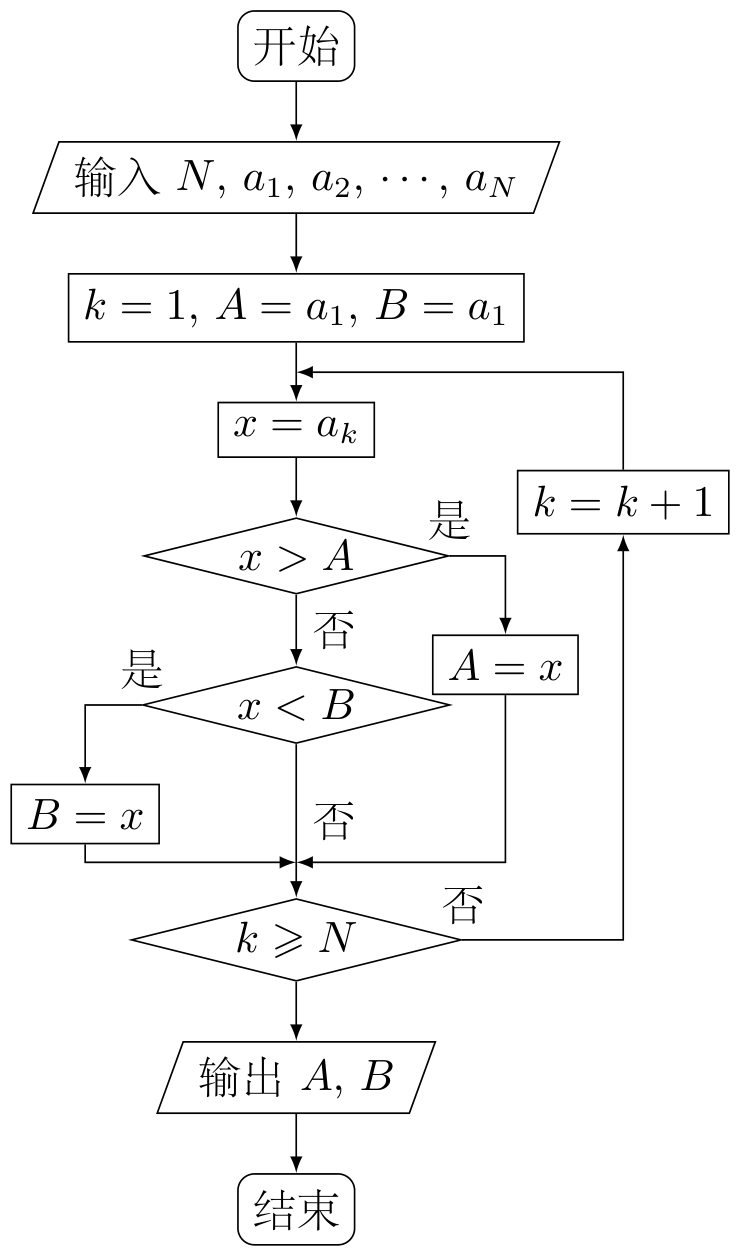
\includegraphics{img/2012/new_curriculum_liberal/q6_fig1.png}}
\bitmapinsertcaption
\end{center}
\endgroup

\choices
    {\(A + B\) 为 \(a_1, a_2, \dots, a_N\) 的和}
    {\(\frac{A + B}{2}\) 为 \(a_1\)，\(a_2\)，\(\dots\)，\(a_N\) 的算术平均数}
    {\(A\) 和 \(B\) 分别是 \(a_1\)，\(a_2\)，\(\dots\)，\(a_N\) 中最大的数和最小的数}
    {\(A\) 和 \(B\) 分别是 \(a_1\)，\(a_2\)，\(\dots\)，\(a_N\) 中最小的数和最大的数}
\end{problem}

\begin{problem}
如图，网格上小正方形的边长为 1，粗线画出的是某几何体的三视图，则此几何体的体积为（\quad）

\bitmapfigure[max width=0.62\linewidth,max totalheight=5.6cm]{img/2012/new_curriculum_liberal/q7_fig1.png}

\choices
    {6}
    {9}
    {12}
    {18}
\end{problem}

\begin{problem}
平面 \(\alpha\) 截球 \(O\) 的球面所得圆的半径为 1，球心 \(O\) 到平面 \(\alpha\) 的距离为 \(\sqrt{2}\)，则此球的体积为（\quad）

\choices
    {\(\sqrt{6}\pi\)}
    {\(4\sqrt{3}\pi\)}
    {\(4\sqrt{6}\pi\)}
    {\(6\sqrt{3}\pi\)}
\end{problem}

\begin{problem}
已知 \(\omega > 0\)，\(0 < \varphi < \pi\)，直线 \(x = \frac{\pi}{4}\) 和 \(x = \frac{5\pi}{4}\) 是函数 \(f(x) = \sin (\omega x + \varphi)\) 图象的两条相邻的对称轴，则 \(\varphi =\)（\quad）

\choices
    {\( \frac{\pi}{4} \)}
    {\( \frac{\pi}{3} \)}
    {\( \frac{\pi}{2} \)}
    {\( \frac{3\pi}{4} \)}
\end{problem}

\begin{problem}
等轴双曲线 C 的中心在原点，焦点在 x 轴上，C 与抛物线 \( y^{2} = 16x \) 的准线交于 A, B 两点，\( |AB| = 4\sqrt{3} \) ，则 C 的实轴长为（\quad）

\choices
    {\(\sqrt{2}\)}
    {\(2\sqrt{2}\)}
    {4}
    {8}
\end{problem}

\begin{problem}
当 \(0 < x \leqslant \frac{1}{2}\) 时，\(4^x < \log_a x\)，则 \(a\) 的取值范围是（\quad）

\choices
    {\(\left(0, \frac{\sqrt{2}}{2}\right)\)}
    {\(\left(\frac{\sqrt{2}}{2}, 1\right)\)}
    {\((1, \sqrt{2})\)}
    {\((\sqrt{2}, 2)\)}
\end{problem}

\begin{problem}
数列 \(\{a_{n}\}\) 满足 \(a_{n + 1} + (-1)^{n}a_{n} = 2n - 1\) ，则 \(\{a_{n}\}\) 的前60项和为（\quad）

\choices
    {3690}
    {3660}
    {1845}
    {1830}
\end{problem}

\section{填空题}

\begin{problem}
曲线 \( y = x(3\ln x + 1) \) 在点(1,1)处的切线方程为\fillinblank{}.
\end{problem}

\begin{problem}
等比数列 \(\{a_{n}\}\) 的前 \(n\) 项和为 \(S_{n}\)，若 \(S_{3} + 3S_{2} = 0\)，则公比 \(q = \)\fillinblank{}.
\end{problem}

\begin{problem}
已知向量 \(a\)，\(b\) 夹角为 \(45^{\circ}\)，且 \(|a| = 1\)，\(|2a - b| = \sqrt{10}\)，则 \(|b| = \)\fillinblank{}.
\end{problem}

\begin{problem}
设函数 \( f(x) = \frac{(x + 1)^2 + \sin x}{x^2 + 1} \) 的最大值为 \(M\)，最小值为 \( m \)，则 \( M + m = \)\fillinblank{}.
\end{problem}

\section{解答题}

\begin{problem}
已知 \(a\)，\(b\)，\(c\) 分别为 \(\triangle ABC\) 三个内角 \(A\)，\(B\)，\(C\) 的对边，\(a \cos C + \sqrt{3} a \sin C - b - c = 0\).
\begin{enumerate}
\item 求 A；
\item 若 \(a = 2\)，\(\triangle ABC\) 的面积为 \(\sqrt{3}\)，求 \(b\)，\(c\).
\end{enumerate}
\end{problem}

\begin{problem}
某花店每天以每枝 5 元的价格从农场购进若干枝玫瑰花，然后以每枝 10 元的价格出售. 如果当天卖不完，剩下的玫瑰花作垃圾处理.
\begin{enumerate}
\item 若花店一天购进 16 枝玫瑰花，卖出的利润 \(y\)（单位：元）关于当天需求量 \(n\)（单位：枝，\(n \in \N\)）的函数解析式；
\item 花店记录了 100 天玫瑰花的需求量（单位：枝）. 整理得下表：
\end{enumerate}

\begin{center}
\renewcommand{\arraystretch}{1.2}
\begin{tabular}{|c|c|c|c|c|c|c|c|}
\hline
日需求量 \(n\) & \(14\) & \(15\) & \(16\) & \(17\) & \(18\) & \(19\) & \(20\) \\
\hline
频数 & \(10\) & \(20\) & \(16\) & \(16\) & \(15\) & \(13\) & \(10\) \\
\hline
\end{tabular}
\end{center}

以 100 天记录的各需求量的频率作为各需求量发生的概率. \circled{1} 假设花店在这 100 天内每天购进 17 枝玫瑰花，求这 100 天的日利润（单位：元）的平均数；\circled{2} 若花店一天购进 17 枝玫瑰花，以 100 天记录的各需求量的频率作为各需求量发生的概率，求当天的利润不少于 75 元的概率.
\end{problem}

\begin{problem}
如图，三棱柱 \(ABC - A_{1}B_{1}C_{1}\) 中，侧棱垂直底面，\(\angle ACB = 90^{\circ}\)，\(AC = BC = \frac{1}{2} AA_{1}\)，\(D\) 是棱 \(AA_{1}\) 的中点.
\begin{enumerate}
\item 证明：平面 \(BDC_{1} \perp\) 平面 \(BDC\)；
\item 平面 \(BDC_{1}\) 分此棱柱为两部分，求这两部分体积的比.
\end{enumerate}

\bitmapfigure[max width=0.44\linewidth,max totalheight=7.0cm]{img/2012/new_curriculum_liberal/q19_fig1.png}
\end{problem}

\begin{problem}
设函数 \( f(x) = \e^{x} - ax - 2 \).
\begin{enumerate}
\item 求 \( f(x) \) 的单调区间；
\item 若 \(a = 1\)，\(k\) 为整数，且当 \(x > 0\) 时，\((x - k)f'(x) + x + 1 > 0\)，求 \(k\) 的最大值.
\end{enumerate}
\end{problem}

\begin{problem}
已知曲线 \(C_1\) 的参数方程是 \(\begin{cases} x = 2\cos \varphi, \\ y = 3\sin \varphi, \end{cases}\) （\(\varphi\) 是参数）以坐标原点为极点，\(x\) 轴的非负半轴为极轴建立极坐标系，曲线 \(C_2\) 的极坐标方程是 \(\rho = 2\). 正方形 \(ABCD\) 的顶点都在 \(C_2\) 上，且 \(A\)，\(B\)，\(C\)，\(D\) 依逆时针次序排列，点 \(A\) 的极坐标为 \(\left(2, \frac{\pi}{3}\right)\).
\begin{enumerate}
\item 求点 A, B, C, D 的直角坐标；
\item 设 \(P\) 为 \(C_{1}\) 上任意一点，求 \(|PA|^{2} + |PB|^{2} + |PC|^{2} + |PD|^{2}\) 的取值范围.
\end{enumerate}
\end{problem}

\begin{problem}
设抛物线 \(C: x^{2} = 2py (p > 0)\) 的焦点为 \(F\)，准线为 \(l\)，\(A\) 为 \(C\) 上一点，已知以 \(F\) 为圆心，\(FA\) 为半径的圆 \(F\) 交 \(l\) 于 \(B\)，\(D\) 两点.
\begin{enumerate}
\item 若 \(\angle BFD = 90^{\circ}\)，\(\triangle ABD\) 的面积为 \(4\sqrt{2}\)，求 \(p\) 的值及圆 \(F\) 的方程；
\item 若 \(A\)，\(B\)，\(F\) 三点在同一直线 \(m\) 上，直线 \(n\) 与 \(m\) 平行，且 \(n\) 与 \(C\) 只有一个公共点，求坐标原点到 \(m\)，\(n\) 距离的比值.
\end{enumerate}
\end{problem}

\begin{problem}
如图，\(D\)，\(E\) 分别为 \(\triangle ABC\) 边 \(AB\)，\(AC\) 的中点，直线 \(DE\) 交 \(\triangle ABC\) 的外接圆于 \(F\)，\(G\) 两点. 若 \(CF // AB\)，证明：
\begin{enumerate}
\item \(CD = BC\)；
\item \(\triangle BCD \sim \triangle GBD\).
\end{enumerate}

\bitmapfigure[max width=0.42\linewidth,max totalheight=5.8cm]{img/2012/new_curriculum_liberal/q22_fig1.png}
\end{problem}

\begin{problem}
已知函数 \( f(x) = |x + a| + |x - 2| \).
\begin{enumerate}
\item 当 a = -3 时，求不等式 \( f(x) \geqslant 3 \) 的解集；
\item 若 \( f(x) \leqslant |x - 4| \) 的解集包含 \( [1, 2] \) ，求 a 的取值范围.
\end{enumerate}
\end{problem}
